% ------------------------------------------
%  IEEE ARTICLE TEMPLATE
% ------------------------------------------
% Author(s):
% Institution(s):
% ------------------------------------------
\documentclass[journal,twocolumn,a4paper,12pt]{IEEEtran}

\usepackage[acronym]{glossaries}
\usepackage[utf8]{inputenc}
\usepackage{ngerman}
\usepackage{hyperref} 
\usepackage{float}
\usepackage{graphicx}
\graphicspath{{figures/}}
\usepackage[german,nameinlink]{cleveref}
\usepackage{url}
\def\UrlBreaks{\do\/\do-}
\usepackage{blindtext}
\usepackage{breqn}
\usepackage{listings}
\lstset{
  columns=fullflexible,
  frame=single,
  breaklines=true,
}

% Use separator for footnotes
\makeatletter
\def\footnoterule{\relax%
	\kern-5pt
	\hbox to \columnwidth{\hfill\vrule width 0.5\columnwidth height 0.4pt\hfill}
	\kern4.6pt}
\makeatother

% Generates the acronyms list
\makeglossaries

% Acronyms list
%!TEX root = ../article.tex

% IEEE
\newacronym{IEEE}{IEEE}{Institute of Electrical and Electronics Engineers}

% ------------------------------------------
%  MAIN DOCUMENT
% ------------------------------------------
\begin{document}
		

% Variables file
%!TEX root = ./article.tex

% Article Title
\def \ArticleTitle{Eine konstruktive Methode zum Rendern von Marching Cubes Voxeln mit unterschiedlichen Füllmengen und Materialien}

% Author(s) Name(s)
\def \AuthorA{Matthias Mettenleiter (\emph{29015})}

% Institution(s) Name(s)
\def \InstitutionA{Studiengang Master Informatik}
\def \InstitutionB{Hochschule Ravensburg-Weingarten}

% Article Title
\newcommand {\Title} {\ArticleTitle}

% Authors
\newcommand {\Authors} {\IEEEauthorblockN{\AuthorA}}

% Institution
\newcommand {\Institutions} {\IEEEauthorblockA{\InstitutionA, \InstitutionB}}

% Variable to control if the bibliography must be include
\def \hasBibliography{1}

% I2C
\newcommand {\interintegratedbus} {I\textsuperscript{2}C}
\newcommand {\itwoc} {\interintegratedbus}
\newcommand{\eeprom}{E\textsuperscript{2}PROM}


% Article title
\title{\Title}

% Author(s) Name
\author{\Authors\\
        \Institutions}

\maketitle

% Abstract
%!TEX root = ../article.tex

% Abstract
\begin{abstract}
Der Marching Cubes Algorithmus ist ein Algorithmus  zur Erzeugung von Oberflächenstrukturen aus Voxeldaten, der im medizinischen Bereich zur Rekonstruktion gemessener 3D-Daten verwendet wird. In diesem Paper wird eine Methode beschrieben, mit dem Marching Cubes Algorithmus, aus konstruierten Voxeldaten, Oberflächen zu rendern. Dazu wird eine Formel vorgestellt, anhand derer beim Erstellen der Marching Cubes die Vertices so verschoben werden, dass die Größe des gerenderten Ergebnisses in Relation zu den Füllmengen der Voxel steht. Auch wird gezeigt, wie unterschiedliche, den Voxeln zugeordnete Materialien auf dem gerenderten Ergebnis über Texturen dargestellt werden können.
\end{abstract}


% Keywords
%%!TEX root = ../article.tex

% Keywords
\begin{IEEEkeywords}
Article, IEEE, template
\end{IEEEkeywords}


% Sections

%!TEX root = ../article.tex

% Entry point for sections:
%
% This file specifies the sections and  its respective order in which they must
% be included.

% Article Sections
%!TEX root = ../article.tex

% Conclusion
\section{Einleitung}
\label{sec:einleitung}
Es gibt verschiedene Methoden Voxel zu rendern. Viele davon werden verwendet um konstruierte Datensätze zu rendern oder auch gemessene Daten zu repräsentieren. Dabei werden Voxel meist binär als gefüllt oder nicht gefüllt unterschieden und entweder mit einer uniformen Größe gerendert oder anhand der gemessenen Werte skaliert. Auch wird diesen oft ein Material zugewiesen, um Voxel unterschiedlich zu nutzen, wie beispielsweise dem Darstellen einer Landschaft oder dem Unterscheiden von Organen in einem medizinischen Scan.

In dieser Arbeit wird eine konstruktive Methode gezeigt Voxel zu rendern, die jeweils eine Füllmenge und ein Material zugewiesen haben. Diese Methode wurde auf Basis eines Projektes entwickelt. \cite{project}
%!TEX root = ../article.tex

% Conclusion
\section{Grundlagen}
\label{sec:grundlagen}

\subsection{Marching Cubes}
\label{subsec:marchingCubes}
Der Marching Cubes Algorithmus wurde entwickelt um gemessene Voxeldaten bei einem medizinischen Scan darzustellen. Beim Marching Cubes Algorithmus werden immer Tupel aus acht Voxeln gebildet, die in kubischer Form angeordnet sind. Bei diesen wird geprüft, ob diese gefüllt sind. Um die gefüllten von den nicht gefüllten Voxeln durch Flächen zu trennen, werden für die jeweilige Konstellation die entsprechenden Vertices aus einer vorgefertigten Lookup-Table erzeugt (siehe Abbildung 1). Dabei liegt ein Vertex immer auf der Kante zwischen den Mittelpunkten eines gefüllten und eines nicht gefüllten Voxels (siehe Abbildung 2). Zur genaueren Repräsentation des gescannten Objektes werden diese Vertices auf der jeweiligen Kante so verschoben, dass ihre Position auf den gemessenen Eintrittspunkten in das gescannte Objekt liegen (siehe Abbildung 3). Sind keine Informationen über die originalen Schnittpunkte vorhanden, so werden die Vertices meist auf der Mitte der Kante platziert. \cite{lorensen1987marching} \cite{iomc} \cite{mc02}

\begin{figure}[H]
			\centering
			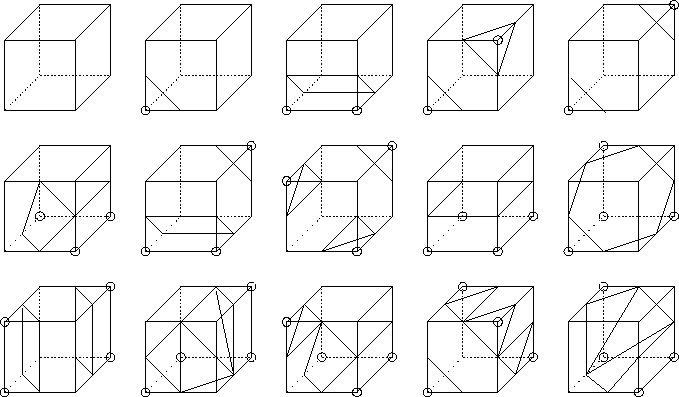
\includegraphics[width=0.5\textwidth]{figures/MarchingCubesPossibilities}
			\caption[Möglichkeiten für MarchingCubes\cite{mc02}]{Möglichkeiten für Marching Cubes \label{MarchingCubesPossibilities}}
		\end{figure}
		
		\begin{minipage}[t]{0.22\textwidth}
			\begin{figure}[H]
			\centering
			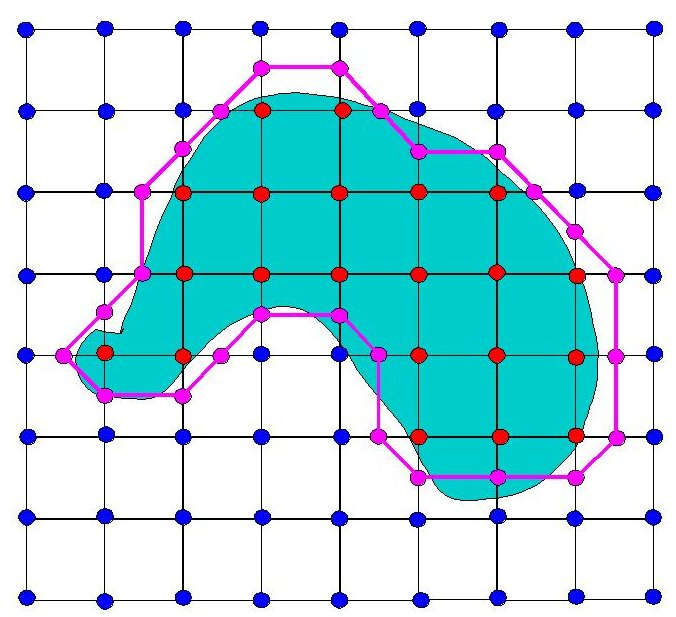
\includegraphics[width=0.98\textwidth]{figures/VerschiebenBeiMarchingCubes1}
			\caption[Marching Cubes Verschiebung (vorher)\cite{iomc}]{Verschiebung bei Marching Cubes (vorher) \label{VerschiebenBeiMarchingCubes1}}
			\end{figure}
			\end{minipage}
			\begin{minipage}[t]{0.22\textwidth}
			\begin{figure}[H]
			\centering
			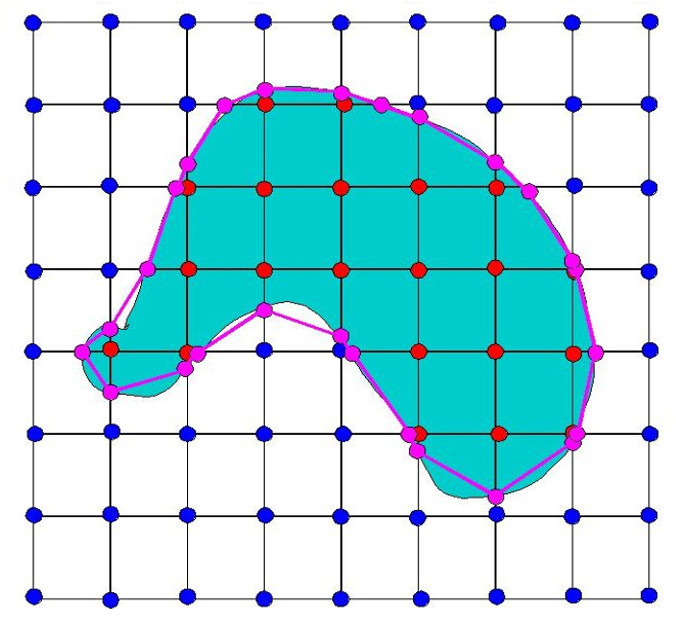
\includegraphics[width=0.98\textwidth]{figures/VerschiebenBeiMarchingCubes2}
			\caption[Marching Cubes Verschiebung (nacher)\cite{iomc}]{Verschiebung bei Marching Cubes (nachher) \label{VerschiebenBeiMarchingCubes2}}
			\end{figure}
			\end{minipage}

\subsection{Material-Interpolation in Marching cubes}
\label{subsec:materialInterpolation}
Eine Methode um Voxel mit jeweils einem Material mit fließenden Übergängen in der Materialdarstellung zwischen unterschiedlichen Materialien zu rendern ist es, den Vertices beim Erstellen jeweils den gefüllten Voxel an der Kante, auf der sie liegen, als primären Voxel zuzuweisen. Somit wird dem jeweiligen Vertex auch das Material des Voxels zugeordnet. Um die Materialien zu interpolieren, werden jedem Vertex die Materialindizes aller Vertices des zu rendernden Polygons und eine Gewichtung für jeden Vertex im Polygon zugewiesen. Durch die Interpolation dieser Werte wird im Polygon bestimmt, welches Material wo gerendert wird. \cite{iomt}

\begin{figure}[H]
			\centering
			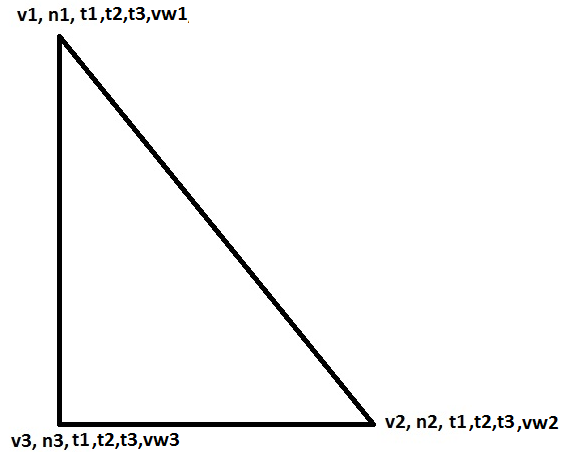
\includegraphics[width=0.3\textwidth]{figures/triangleCorrected}
			\caption[Polygon mit zusätzlichen Werten zur Interpolation\cite{iomt}]{Polygon mit zusätzlichen Werten zur Interpolation: (v*) Vertex Position, (n*) Normale, (t1, t2 und t3) Materialien der drei Richtungen, (vw*) Gewicht der Materialien am Vertex \label{PolygonMitZusatzWerten}}
			\end{figure}

\subsection{Triplanares Mapping}
\label{subsec:triplanaresMapping}
Um zweidimensionale Texturen ohne Verzerrungen und ohne unterschiedliche Detailgrade auf ein beliebiges Objekt zu mappen, wird Triplanares Mapping verwendet. Hierzu werden die dreidimensionalen Positionen innerhalb des Objektes in die drei planaren Projektionen aus Richtung der Hauptachsen aufgeteilt. Für die drei so erzeugten zweidimensionalen Positionen wird jeweils die Farbe aus der Textur gesucht. Die drei so erhaltenen Werte werden anhand der Werte der Normalen des Polygons an der jeweiligen Position gemischt. \cite{tpm}




%!TEX root = ../article.tex

% Conclusion
\section{Zielsetzung}
\label{sec:zielsetzung}
Das Ziel dieser Arbeit ist eine Methode zu zeigen, die den Marching Cubes Algorithmus verwendet, um Oberflächen für Voxel zu erzeugen, die konstruktiv erzeugt werden und nicht aus Messdaten hervorgehen. Die erzeugten Daten sollen dabei unterschiedliche Materialien enthalten und nicht binär in gefüllt und nicht gefüllt unterschieden werden, sondern eine kontinuierliche Füllmenge aufweisen. Folgende Anforderungen werden dabei gestellt:
\begin{itemize}
\item Jedem Voxel werden ein Material und eine kontinuierliche $F"ullmenge \in [1,0]$ zugewiesen. 
\item Es wird pro Achter-Tupel (siehe \ref{subsec:marchingCubes}) ein Mesh erzeugt. Hierbei haben die einzelnen Voxel nur Zugriff auf die ihnen zugewiesenen Informationen und keine Referenzen oder Zugriffe auf andere Voxel, wie beispielsweise ihre sechs direkten Nachbarn.
\item Die Größe der Meshes wird sich anhand der Füllmenge innerhalb eines Voxels verändern und nachvollziehbar sein. Nachvollziehbar bedeutet in diesem Zusammenhang, dass bei mehr Füllmenge ein größerer Mesh entsteht und umgekehrt. Es ist in diesem Fall keine Anforderung, dass die Ausdehnung volumetrisch korrekt ist.
\item Es ist möglich ein Objekt zu erzeugen, das nur aus waagerechten und senkrechten Flächen besteht. Daraus geht hervor, dass es möglich ist 90$^\circ$ Außenwinkel aus senkrechten und waagerechten Flächen zu erzeugen.
\item Da durch die Skalierung der Marching Cubes unterschiedlich große Flächen in den Meshes entstehen, wird Solid Texturing verwendet, um unterschiedliche Detailgrade zu vermeiden.
\item Es werden fließende Übergänge zwischen den Texturen der verschiedenen Materialien gerendert. Dabei werden ebenfalls nur die Daten der acht Voxel verwendet, die zum Finden der Marching Cubes Variante in der Lookup-Table benötigt werden.
\item Die Füllmenge eines Voxels beeinflusst auch, wie das Material des Voxels im Verhältnis zu den Materialien der Nachbarn in den Texturübergängen gemischt wird.
\end{itemize}
%!TEX root = ../article.tex

% Conclusion
\section{Aufbau der Voxelstruktur}
\label{sec:aufbauVoxelstruktur}
Jeder Voxel enthält einen Wert, der den Materialtyp des Voxels definiert und eine $F"ullmenge \in [1,0]$.

Die Voxel befinden sich in einer übergeordneten Struktur, anhand dieser deren Position definiert ist.

Ein Voxel hat selbst keine direkten Informationen über seine Nachbarn, jedoch enthält jeder Voxel zusätzlich die Information darüber, wie viele seiner sechs Nachbarn gefüllt sind. Diese Information lässt Abhängigkeiten der Ausdehnung des Meshes von der Umgebung des Voxels zu, ohne dass beim Erstellen des Meshes die Nachbarn betrachtet werden müssen. Auch wird anhand der Information geprüft, ob er von allen Seiten mit gefüllten Voxeln umgeben ist. Ist dies der Fall, ist der Voxel nicht sichtbar und wird nicht gerendert. Jedes Mal wenn sich der Status eines Voxels von gefüllt zu nicht gefüllt oder umgekehrt ändert, werden alle Nachbarn über diese Änderung informiert und passen so ihre Menge gefüllter Nachbarn an.

%!TEX root = ../article.tex

% Conclusion
\section{Implementierung der  Oberflächengenerierung}
\label{sec:implementierungOberflaeche}
Die Vertices bei der Erstellung eines Marching Cubes Meshes werden immer auf einer Kante zwischen zwei Voxeln innerhalb  des Achter-Tupels platziert. Dabei liegt ein solcher Vertex immer zwischen einem gefüllten und einem nicht gefüllten Voxel, um diese zu trennen. (siehe \ref{subsec:marchingCubes})

Um die Meshes unterschiedlich groß in Relation zu der Füllmengen der gerenderten Voxel zu Rendern, wird eine Ausdehnung eingeführt, die sich durch den Abstand zum Mittelpunkt eines Voxels definiert. Die Ausdehnung ist 0, wenn sich der Vertex direkt beim Voxel befindet und die Ausdehnung ist 1, wenn sich der Vertex die Gesamtlänge einer Kante zu einem benachbarten Voxel entfernt befndet.

Auch wird ein Schwellwert eingeführt, um zu bestimmen, ab wann der Voxel für das Generieren des Meshes aus der Lookup-Table als gefüllt gewertet wird.

Das Verhältnis der Füllmengen der zwei Voxel auf einer Kante, auf der sich ein Vertex befindet, wird verwendet, um zu bestimmen, wann sich dieser Vertex ganz bei dem gefüllten Voxel befindet und wie die Ausdehnung von diesem ausgehend berechnet wird.

\subsection{Schwellwerte zum Rendern der Voxel}
Das Volumen zwischen den Mittelpunkten achter kubisch angeordneten Voxel wird als Einheitsmenge 1 definiert, so dass jedes Achter-Tupel zwischen seinen Mittelpunkten eine Einheitsmenge enthält.

Wird ein Objekt erzeugt, das aus acht kubisch angeordneten Voxeln mit jeweils gleicher Füllmenge besteht, die nur von leeren Voxeln umgeben sind und das nur aus waagerechten und senkrechten Flächen besteht, entsteht ein Würfel, der diese Einheitsmenge einschließt.

Dabei sind die Vertices der Marching Cubes auf ihren Kanten jeweils direkt bei den gefüllten Voxeln und besitzen damit die Ausdehnung 0.

Um dieses Volumen aus den Füllmengen der acht Voxel zu generieren, muss jeder Voxel in der beschriebenen Struktur die Füllmenge 1/8 besitzen.

Ein solcher Würfel besitzt demnach eine Ausdehnung von 0 um die zu 1/8 gefüllten Voxel und ein Volumen von 1. Um nachvollziehbar zu sein wird sich das Objekt verkleinern, wenn bei diesem Würfel aus einem Voxel Material entnommen wird.

Daraus geht hervor, dass die Voxel mit einer kleineren Füllmenge als dieser Schwellwert zum Rendern als nicht gefüllt betrachtet werden.

Wird der Würfel um vier Voxel erweitert, so dass sich ein Quader ergibt, so ist dessen Volumen Zwei. Es ist für die Füllmengen zu beachten, dass bei den Voxeln, die neue Nachbarn erhalten haben, auch neue Verbindungen entstehen. Aufgrund dessen wird der Schwellwert in Abhängigkeit der Menge gefüllter Nachbarn gesetzt, die innerhalb eines jeden Voxels vermerkt sind. (Siehe Abschnitt \ref{sec:aufbauVoxelstruktur})
\\

Die Formel zur Bildung der Schwellwerte ist
\[s = \frac{1}{(l)^{2}}\]
wobei $s$ = Schwellwert und $l$ = Anzahl der sechs direkten Nachbarn, die nicht gefüllt sind. Da der Voxel komplett verdeckt ist und somit nicht gerendert wird, wenn er nur gefüllte Nachbarn besitzt, gibt es keine Probleme mit dem dabei entstehenden Nullteiler.

\subsection{Berechnung der Ausdehnung ausgehend vom gefüllten Voxel}
Zuerst wird eine Grundausdehnung durch die Füllmenge des gefüllten Voxels bestimmt. Diese ist 0, wenn sich die Füllmenge des gefüllten Voxels genau an seinem Schwellwert befindet. Um wieder die Einheitsgröße 1 als Volumen zwischen den Mittelpunkten von acht kubisch angeordneten Voxeln zu beachten wird die maximale Grundausdehnung eines komplett gefüllten Voxels auf $\frac{\sqrt{2}}{2}$ gesetzt. Der Diamant, der entsteht, wenn ein komplett gefüllter Voxel nur von leeren Voxeln umgeben ist, hat dadurch eine Kantenlänge von 1 und ebenfalls das Volumen 1.

Die Gesamtausdehnung entsteht, indem die Grundausdehnung graduell anhand der Füllmenge des nicht gefüllten Voxels so aufgefüllt wird, dass ein fließender Übergang zu dem Zustand entsteht, an dem der nicht gefüllte Voxel seinen Schwellwert erreicht.
\\

Die Grundausdehnung berechnet sich über die Formel
\[a_g= \frac{f_g-s_g}{1-s_g}*\frac{\sqrt{2}}{2}\]
wobei $a_g$ = Grundausdehnung, $f_g$ = Füllmenge des gefüllten Voxels und $s_g$ = Schwellwert, des gefüllten Voxels.
\\

Daraus berechnet sich dann die Gesammtausdehnung über die Formel
\[a = a_g + \frac{1}{a_g} * \frac{f_n}{s_n}\]
wobei a = Gesammtausdehnung, $a_g$ = Grundausdehnung, $f_n$ = Füllmenge des nicht gefüllten Voxels und $s_n$ = Schwellwert, des nicht gefüllten Voxels.
%!TEX root = ../article.tex

% Conclusion
\section{Implementierung der  Texturierung}
\label{sec:implementierungTexturierung}
Da bei einem Vertex, der zwischen zwei Voxeln liegt, die beide eine Füllmenge > 0 haben das Meterial beider Voxel beim Texturieren beachtet werden soll kann nicht jedem Vertex ein primärer Voxel zugewiesen werden, wie in Abschnitt \ref{subsec:materialInterpolation} beschrieben.

Die Mischverhältnisse der Materialien werden daher anhand der Position innerhalb des jeweiligen Achter-Tupels bestimmt. Dabei haben die Füllmengen der Voxel ebenfalls eine Auswirkung auf diese Mischverhältnisse.
\\

Der Abstand zu jedem Voxel im Achter-Tupel berechnet sich über folgende Formel (Dabei sind die acht Voxel innerhalb des Tupels über $i \in [0,7]$ nummeriert)
\[a_i= dif(x_i,x)*dif(y_i,y)*dif(z_i,z)\]
wobei $a_i$ = Abstand vom $i$ten Voxel, $(x,y,z)$ = Position innerhalb des Tupels, $(x_i,y_i,z_i)$ Position des $i$ten Voxels innerhalb des Tupels und $dif(a,b)$ = Differenz zwischen $a$ und $b$.
\\

Die Materialmischung berechnet sich über die Formel
\[m = \frac{\sum\limits_{i=0}^{7}m_i*a_i*f_i}{\sum\limits_{i=0}^{7}a_i*f_i}\]
wobei $m$ = Mischmaterial, $m_i$ = Materialeigenschaft (z.B.Farbe)  des $i$ten Voxels, $a_i$ = Abstand vom $i$ten Voxel und $f_i$ = Füllmenge des $i$ten Voxels.
%!TEX root = ../article.tex

% Conclusion
\section{Fazit}
\label{sec:fazit}
Die gezeigte Methode ermöglicht unterschiedlich große und komplexe Oberflächen über den Marching Cubes Algorithmus zu rendern, die aus einer konstruierten Voxelstruktur mit dynamischen Füllmengen und unterschiedlichen Materialien bestehen. Dabei werden sämtliche gestellte Anforderungen erfüllt.

\begin{figure}[H]
			\centering
			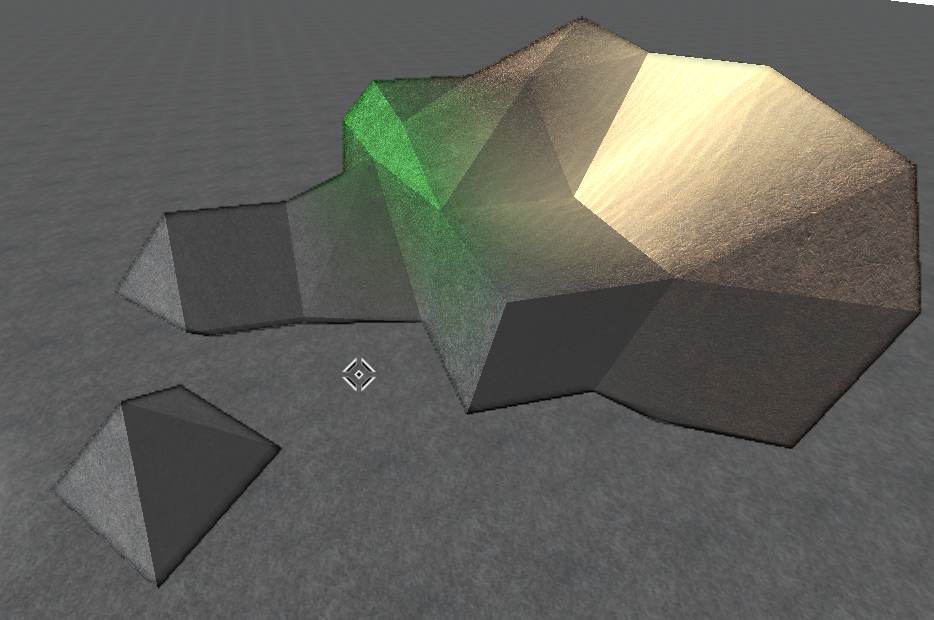
\includegraphics[width=0.5\textwidth]{figures/ProjectImage}
			\caption[Beispiel aus dem Projekt\cite{project}]{Beispiel aus dem Projekt \label{MarchingCubesPossibilities}}
\end{figure}
%!TEX root = ../article.tex

% Conclusion
\section{Ausblick}
\label{sec:ausblick}
Diese Methode ist noch erweiterbar und es können weitere Verfeinerungen vorgenommen werden. Ein paar der weiteren Ansätze wären:
\begin{itemize}
\item Die Lookup-Table kann angepasst werden, um die Trennung der gefüllten von den nicht gefüllten Voxeln über andere Oberflächen vorzunehmen. Dabei ist es denkbar, zu berücksichtigen, wie sich unterschiedliche Materialien zueinander verhalten. So kann eine Methode entwickelt werden, gleichartige Materialien zu verbinden und unterschiedliche Materialien zu trennen. Dazu ist auch zu beachten, wie sich die Übergänge zwischen den Materialien an solchen Stellen verhalten.
\item Die Normalen an den Vertices können  so angepasst werden, dass ein eher fließender Übergang an den Kanten stattfindet, der die Beleuchtung beeinflusst. Dieses Verhalten könnte vom Winkel zwischen den Flächen an den Kanten abhängig gemacht werden. Es ist auch hier möglich dieses Verhalten von den Materialien abhängig zu machen, so dass es Materialien mit härteren Kanten und weicheren Kanten gibt.
\item Es ist denkbar, nicht ein Material pro Voxel zu verwenden, sondern verschiedene Mengen an verschiedenen Materialien innerhalb eines Voxels zu definieren, deren Gesamtmenge dann der Füllmenge entsprechen würde. Dazu muss die Methode zum Darstellen der Texturen auf den Voxeln angepasst werden. \cite{rvmm}
\item Den Materialien könnten noch renderspezifische Verhaltensweisen wie unterschiedliches Beleuchtungsverhalten oder Reflektionen zugewiesen werden.
\item Es gibt Methodem dazu, Normal Mapping mit Triplanarem Mapping zu verbinden. Diese Ansätze ließen sich mit den Ergebnissen dieser Arbeit vereinen. \cite{nmfts}
\item Verschiedene Methoden Schatten zu berechnen, können im Zusammenhang mit dieser Methode getestet werden.
\item Es ist denkbar zu versuchen die Methode so anzupassen, dass die Ausdehnung der Objekte im Verhältnis zu den Füllmengen der Voxel volumetrisch korrekt gerendert wird.
\end{itemize}


%%!TEX root = ../article.tex

% Introduction
\section{Vorgehen}
Um mögliche Auswirkungen einer EDID-Manipulation reproduzierbar prüfen zu können, wird ein Testsystem benötigt. Hierfür wurde ein \emph{Raspberry Pi 3B} mit Raspbian als Betriebssystem sowie ein \emph{ATmega2560} Microcontroller (Elegoo MEGA 2560 R3) zusammen mit einem HDMI Breakout-Board eingesetzt. Damit lässt sich ein Monitor simulieren indem der Raspberry die EDID-Daten über den \interintegratedbus-Bus anfragt und von dem Microcontroller geliefert bekommt. 

Auf diese Weise besteht die Möglichkeit die EDID-Verarbeitung nicht nur direkt zu testen sondern, aufgrund der Quelloffenheit von Linux, auch direkt im Quelltext statisch zu analysieren.

\subsection{Versuchsaufbau}
Der Versuchsaufbau konzentriert sich auf Plug\&Play sowie die Übertragung von EDID-Blöcken über \interintegratedbus. 
Aus diesem Grund werden nicht alle HDMI Pins genutzt. Tabelle \ref{TblRelevantePins} stellt die relevanten Pins für diesen Aufbau dar. 
Wie sich dieser Versuchsaufbau erweitern ließe wird in \cref{sec:ausblick} skizziert.


\hspace*{-4cm}
\begin{table}[H]
	\caption{Genutzte Pins des HDMI Ports}
	\def\arraystretch{1.5}
	\centering
	\small
	\setlength\tabcolsep{1pt}
	\label{TblRelevantePins}
	\makebox[-1.1 \textwidth][c]{       %centering table
\begin{tabular}{|c|c|c|}
	\hline 
	\textbf{Pin} & \textbf{Funktion} & \textbf{Beschreibung}\\ 	\hline 
	15 & SCL & Clock-Signal für den \interintegratedbus-Bus\\ \hline 
	16 & SDA & Datenlinie für den \interintegratedbus-Bus\\ \hline 
	17 & DDC/CEC Ground & Einheitliche Erde\\ \hline 
	18 & +5V & Spannungsversorgung für \interintegratedbus und den \eeprom \\ \hline 	
	19 & Hot-Plug-Detect & HIGH für 'an', LOW für 'aus'\\ \hline 		
\end{tabular} 
}
\end{table}

Diese Pins müssen entsprechend Abbildung \ref{fig:hdmi-arduino} mit dem Microcontroller 
verschaltet werden\footnote{Die gesamte Pinbelegung kann in der HDMI Spezifikation nachgelesen werden (\cite[S.12]{Hdmi14Specification})}. \newpage

Die SCL- und SDA-Pins werden direkt mit den entsprechenden Pins auf dem Arduino-Board  verbunden.
Das selbe gilt für die Pins 17 und 18. Diese werden mit die GND und 5V-Pins verbunden. 
Der Hotplug-Pin kann mit einem beliebigen digitalen Ausgangspin verschaltet werden. 
Wird er auf \emph{High} gesetzt, wird das Kabel ``eingesteckt'' und analog bei \emph{Low} ``ausgesteckt''.
Hier müssen die --- von der HDMI Spezifikation vorgegebenen --- Zeiten eingehalten werden \cite[S.73]{Hdmi14Specification}.
Die dargestellten Widerstände können genutzt werden, dazu müssen die internen Pull-Up Widerstände des Arduino allerdings ausgeschaltet werden. 
Ansonsten können die Widerstände auch weggelassen werden.

\begin{figure}[H]
	\centering
	\includegraphics[width=0.5\textwidth]{hdmi-arduino}
	\caption{Verschaltung HDMI und Arduino MEGA 2560}
	\label{fig:hdmi-arduino}
\end{figure}

\subsection{Microcontroller Software}
Auf dem Microcontroller befindet sich ein Programm welches den Hot-Plug-Pin setzen kann. Über eine serielle Schnittstelle kann der Pin  geschaltet werden ohne den Versuchsaufbau 
verändern zu müssen.
Somit kann der Versuchsaufbau stehen bleiben ohne Kabel ein- und aus-stecken zu müssen. Dieses Programm kümmert sich außerdem um die Verarbeitung des \acrshort{ddc}. 
Wenn die EDID-Daten vom Host angefragt werden so sorgt es dafür, dass diese \interintegratedbus-Anfragen entsprechend beantwortet werden. Es liefert zunächst nur einen
Standard-EDID Block ohne Extensions zurück. Je nach Konfiguration können allerdings Extension-Blöcke gesendet werden. 
Des Weiteren ermöglicht es das Programm die einzelnen Bytes des 128 Byte langen EDID-Blocks frei zu verändern und korrigiert entsprechend das Prüfsummen-Byte des Blocks.

\subsection{Statische Analyse}
Zusammen mit dem Versuchsaufbau wird eine statische Analyse des Quellcodes der betroffenen Module durchgeführt. Dies ermöglicht das direkte überprüfen sowie einen umfassenden Einblick
aufgrund der Quelloffenheit von Linux.

Für den X-Server findet sich die Implementierung von \acrshort{ddc} in \path{hw/xfree86/ddc/} sowie \path{hw/xfree86/common/}\footnote{Siehe: \url{https://github.com/mirror/xserver}}.
Die entsprechende Implementierung von \acrshort{ddc} für das DRM Subsystem des Kernels liegt in \path{drivers/gpu/drm}\footnote{Siehe: \url{https://github.com/torvalds/linux}}

Durch diese Kombination wurde ein Testaufbau erzeugt welcher sowohl die konkrete Implementierung untersuchbar macht als auch die direkte Überprüfung von Vermutungen ermöglicht.
Im nächsten Abschnitt wird dabei genauer auf die Funktionsweise des Codes eingegangen. 






%%!TEX root = ../article.tex

% Conclusion
\section{Ergebnisse}
\label{sec:conclusion}

\subsection{EDID-Verarbeitung in xfree86 DDX}
Die Verarbeitung beginnt in \texttt{hw/xfree86/ddc/ddc.c}. In diesem Modul wird die Funktion \texttt{xf86DoEEDID()} aufgerufen, welche über den \interintegratedbus-Bus 128 Byte Blöcke einliest.
Die \textbf{Prüfsumme} der eingelesenen EDID-Blöcke wird direkt nach dem Einlesen überprüft. Ist diese nicht korrekt wird der Block verworfen und nicht verarbeitet. So ist für einen eventuellen Angriff auf jeden Fall 
eine korrekte Prüfsumme erforderlich.
Nach dem Lesen wird ein 128 Byte Speicherbereich für den ersten Block angelegt und darin gespeichert. 
Aus diesem Block wird die Anzahl der Extension-Blöcke gelesen damit diese ebenfalls gelesen werden können. 
Vor dem Einlesen wird der bereits allozierte Speicherbereich um die Anzahl der Extension-Blöcke (auch mit stets 128 Byte) vergrößert.

\begin{itemize}
	\item Zunächst wird die  \textbf{Vendor-Section} (Byte 8-17, little endian)\footnote{Alle Angaben beziehen sich auf den EDID Standard 1.3. Siehe \cite[S.9ff]{Edid13Specification}} verarbeitet.
	Bit 15 ist dabei für zukünftige Verwendung reserviert, wird aber in der Verarbeitung gar nicht beachtet, sodass hier kein Angriff möglich ist. 
	Die folgenden zwei Bytes enthalten die von Microsoft vorgegebenen PNP-IDs, die den Hersteller eines Plug-and-Play Geräts angeben. Es ist festzustellen, dass nicht alle Bit-Permutationen definiert sind, da die genutzte Codierung nicht die gesamten 16 Bit benötigt. Dennoch war auf dem Testsystem bei setzen nicht definierter Werte kein abweichendes Verhalten festzustellen, da nicht-passende Bytes ersetzt werden.
	Das Produktionsjahr (Byte 16) erlaubt  nur Werte zwischen 0 und 53 (\cite[S.11]{Edid13Specification}). Dennoch haben auch hier abweichende Werte keine feststellbaren Auswirkungen.
	\item Version und Revision (Byte 18-19) werden lediglich in das, dem Treiber zur Verfügung gestellte, struct geschrieben und nicht weiter geprüft. 
	\item 	Die nächsten 15 Byte beinhalten weitere Informationen zum Display.
	In Byte 20 Bit sieben wird dabei angegeben, ob das Display analog oder Digital betrieben wird. Davon hängt ab, ob die Bits null bis sechs verwendet werden müssen oder nicht. Bei analogem Betrieb ist dies der Fall, bei digitalem nicht. Dann muss laut HDMI-Spezifikation(Verweis einfügen) bei allen Werten der Default Wert null gesetzt werden. Dies geschieht allerdings nicht. Hier sollte daher der Treiber eine Überprüfung durchführen. Die restlichen Bytes werden ohne Überprüfung geschrieben.
	\item 	Die nächsten drei Bytes geben an, welche Auflösungen bei welcher Frequenz vom Bildschirm unterstützt werden. Dabei sind in den ersten beiden Bytes je eine Auflösung an ein Bit gebunden. Diese werden ohne Überprüfung akzeptiert. Ein Angriff ist hier erstmal nicht möglich. Im dritten Byte ist ein Bit für eine weitere Auflösung vorgesehen, die restlichen 6 Bit können vom Bildschirmhersteller frei gesetzt werden. Hier ist wieder auschlaggebend, wie und ob der Treiber diese Bits beachtet.
	\item Die darauf folgenden 16 Byte enthalten die Standard Timing Information und sind aufgeteilt in acht zwei-Byte Blöcke. Jeder Block wird auf Validität geprüft. Dabei Darf nicht in beiden Byte der Wert 0x01, 0x00, 0x20 enthalten sein. Ist dies der Fall, werden alle Werte auf 0 gesetzt.
	\item 	Die nächsten 72 Bytes enthalten die Detailed Timing Sections. Diese sind aufgeteilt in vier Descriptoren  mit je 18 Byte. Hier wird zuerst geprüft, ob die EDID-Version gleich eins und die Revision größer null ist. Dies ermöglicht unter umständen einen Angriff, da beim Auslesen der Version und Revision keine Plausibilitätsprüfung unternommen wird. Des Weiteren wird Überprüft, ob der Descriptor ein Timing oder ein Other Monitor Descriptor ist.
	Ist die EDID-Version größer 1.0 wird zwischen verschiedenen Descriptoren unterschieden und die Daten entsprechend des jeweiligen Descriptoren geschrieben. Ansonsten werden die Daten ungeprüft nach festem Schema geschrieben. 
	Die Daten eines Other Monitor Descriptors werden ohne Überprüfung akzeptiert. Dies ist insofern Interessant, als dass hier der Hersteller oder Angreifer 13 Byte zur Verfügung hat, in die er schreiben kann was er möchte. Jedoch ist keine Längenangabe notwendig, die manipuliert werden könnte. Es sind maximal 13 Bytes erlaubt.
	
	
\end{itemize}





\subsection{EDID-Verarbeitung in DRM}
Eine weitere EDID-Verarbeitung findet sich im Kernel-Modul DRM. Diese wird von DRM-Treibern verwendet. 

Zu Beginn wird der Base-Block eingelesen und validiert. Dabei werden maximal vier Versuche gestartet.  War dann kein Einlesen und keine Validierung erfolgreich, wird der Versuch abgebrochen und NULL zurück gegeben.

Die Validierung besteht aus folgenden Prüfungen:
Der EDID-Header, also die ersten acht Bytes, muss stimmten. Ist dies der Fall, wird die Checksumme des Blockes überprüft. Ist auch diese korrekt, muss die Version kleiner 1.5 sein. Nur wenn alle Bedingungen wahr sind, wird der Block als zulässig akzeptiert. Ansonsten ist er ungültig und wird verworfen.

Wenn der Base-Block gültig ist, wird Speicherplatz für die im Base-Block angegebene Anzahl Extension-Blöcke allokiert sofern solche Blöcke vorhanden sind. Dieser Speicherplatz wird wieder freigegeben, sobald ein Fehler auftritt und NULL zurück gegeben wird. Hierüber ist also kein Angriff möglich.
Anschließend werden die  Extension-Blöcke eingelesen und verarbeitet. Diese werden nacheinander eingelesen, wobei für jeden Block vier versuche gestartet werden. Dabei ist die Anzahl der Versuche fest codiert und nicht von einer Variable abhängig. Jeder Extension-Block wird auf Validität geprüft.
Dabei wird nur die Checksumme geprüft.
Sind alle Extension-Blöcke überprüft und die nicht validen aussortiert, wird der allokierte Speicher reallokiert sodass er auf die Anzahl und damit die Speichergröße der validen Blöcke passt. Außerdem wird die Anzahl der Extension-Blöcke im Base-Block angepasst damit es später zu keinem Fehler kommt.
Dies ist die komplette EDID-Verarbeitung im Kernel. Die eigentliche Interpretation der Daten erfolgt erst im Treiber.

\subsection{Windows}
Zu Beginn des Projekts wurde getestet, ob der simulierte Bildschirm auch von Windows erkannt wurde. Er wird erkannt, jedoch werden die Extension-Blöcke von Windows nicht beachtet. Nur der Base-Block wird von Windows selbst in die Registry geschrieben. Daher wird ein Angriff deutlich schwieriger, da die Extension-Blöcke mehr Möglichkeiten bieten, Daten zu manipulieren.

\subsection{Verhalten RaspberryPi}	HDMI hat einen integrierten Hot-Plug-Pin. Mit diesem kann ein Connector aus- oder eingesteckt werden, ohne das die eigentliche Steckverbindung gelöst werden müsste.
Unter Windows funktioniert dies tadellos und wird jedes mal richtig erkannt.
Unter Raspbian auf dem Raspberry Pi ist dies nicht der Fall. Dort wird beim ``Ausstecken'', also durch senden einer logischen Null durch den Hot-Plug-Pin der Bildschirm zwar als ausgesteckt erkannt. Wird er jedoch durch setzen einer logischen Eins auf dem Hot-Plug-Pin wieder eingesteckt, wird das Display nicht jedes mal erkannt. 
Durch Versuche konnte kein einheitliches Verhalten festgestellt werden. Teilweise wurde das Display beim ersten Versuch erkannt, teilweise erst beim sechsten.
Durch dieses Verhalten wird Fuzzing extrem erschwert, da der HDMI Connector bei jedem Versuch aus und wieder eingesteckt werden müsste.


\subsection{Reproduzierbarkeit}
Ein Angriff auf ein System mithilfe einer Manipulation von EDID-Daten ist aufgrund der unterschiedlichen Verarbeitungswege nicht auf andere Betriebssysteme, auch nicht bedingungslos auf andere Linux-Systeme, übertragbar. Die Windows-Verarbeitung wurde für dieses Dokument gar nicht weiter untersucht.
Auch ist ein möglicher Angriff auf einen DRM-Treiber nicht auf andere DRM-Treiber übertragbar, da diese bei der EDID-Verarbeitung sehr viel selbst übernehmen und nicht auf standardisierte Kernel-Funktionen zurück greifen. 


%\printglossaries



\addcontentsline{toc}{section}{Abbildungsverzeichnis}
\listoffigures

\bibliographystyle{plain}
\bibliography{bibliography/article}

\end{document}
